\noindent

\includegraphics[height=1.25cm]{images/pictograms/replication}

\includegraphics[height=1.25cm]{images/pictograms/benchmark}

\includegraphics[height=1.25cm]{images/pictograms/FEM}

\includegraphics[height=1.25cm]{images/pictograms/paraview}

%%%%%%%%%%%%%%%%%%%%%%%%%%%%%%%%%%%%%%%%%%%%%%%%%%%%%%%%%%%%%%%%%%%%%%%%%%%%%%%%%%%%%%%%%%%%%%%%%%%

\begin{flushright} {\tiny {\color{gray} python\_codes/fieldstone\_181/text.tex}} \end{flushright}

%\lstinputlisting[language=bash,basicstyle=\small]{python_codes/template_keywords.key}

\par\noindent\rule{\textwidth}{0.4pt}

\begin{center}
\inpython
{\small Code: \url{https://github.com/cedrict/fieldstone/tree/master/python_codes/fieldstone_181}}
\end{center}

\par\noindent\rule{\textwidth}{0.4pt}

Last revision: September 18th, 2025.

\par\noindent\rule{\textwidth}{0.4pt}

%%%%%%%%%%%%%%%%%%%%%%%%%%%%%%%%%%%%%%%%%%%%%%%%%%%%%%%%%%%%%%%%%%%%%%%%%%%%%%%%%%%%%%%%%%%%%%%%%%%

This \stone is a new take on \stone~40. 
The setup is identical. We here focus on the assembly of the FE matrix. 
Three methods are implemented and timed:
\begin{enumerate}
%-------------------------------------------------------------
\item The first one relies of defining the matrix as a linked list:
\begin{lstlisting}
A_fem=lil_matrix((Nfem,Nfem),dtype=np.float64)
\end{lstlisting}
The boundary conditions and assembly process are rather straightforward
looping over all elements, their velocity and pressure dofs.
Finally the matrix is converted to the CSR format:
\begin{lstlisting}
A_fem=sps.csr_matrix(A_fem)
\end{lstlisting}



%-------------------------------------------------------------
\item The second one has already been explored in \stone~150.
It relies on 3 large arrays:
\begin{lstlisting}
bignb=nel*((m_V*ndof_V)**2+2*(m_V*ndof_V*m_P))
II_V=np.zeros(bignb,dtype=np.int32)    
JJ_V=np.zeros(bignb,dtype=np.int32)    
VV_V=np.zeros(bignb,dtype=np.float64)    
\end{lstlisting}
The first two are filled before the loop over 
elements and contain indices of nonzeros. 
The third is filled with the $\K_e$ and $\G_e$ matrices.
Finally the matrix is converted to csr as follows:
\begin{lstlisting}
A_fem=sps.coo_matrix((VV_V,(II_V,JJ_V)),shape=(Nfem,Nfem)).tocsr()
\end{lstlisting}

%-------------------------------------------------------------
\item The third one is probably the simplest. It is presented in 
\stone~176 for the $Q_1\times P_0$+penalty case.
The matrix and indexing arrays are simply defined as follows:
\begin{lstlisting}
row=[] 
col=[]
A_fem=[]
\end{lstlisting}
The elemental matrices (and the corresponding dofs) 
are then appended one component at a time to these arrays. 
Finally the matrix is converted to csr as follows:
\begin{lstlisting}
A_fem=sps.csr_matrix((A_fem,(row,col)),shape=(Nfem,Nfem))
\end{lstlisting}
 
\end{enumerate}

For all three methods we will measure various times as a function 
of matrix size \lstinline{Nfem}, i.e. 

\begin{itemize}
\item The total time taken to build the FE system: 
\begin{center}
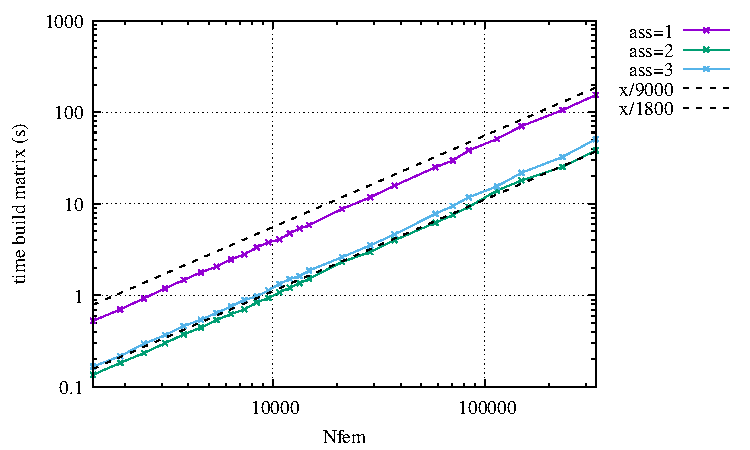
\includegraphics[width=10cm]{python_codes/fieldstone_181/RESULTS/times_build.pdf}
\end{center}
\item The total time spent in the assembly alone. In all three cases it scales 
linearly with the number of dofs, but method 2 is more than 10x faster than method 1. 
\begin{center}
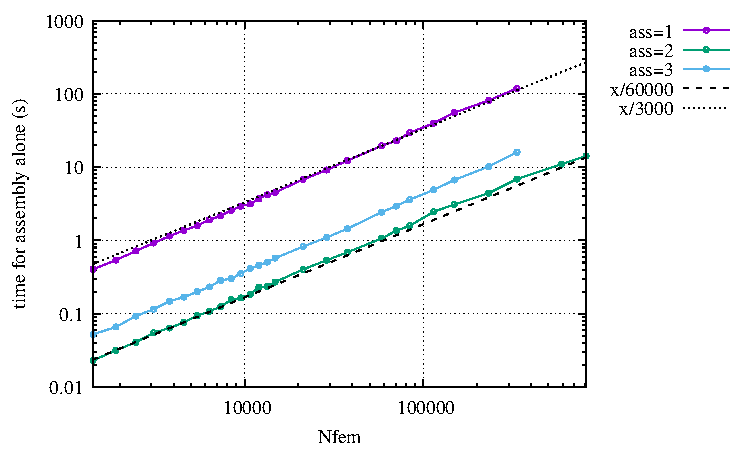
\includegraphics[width=10cm]{python_codes/fieldstone_181/RESULTS/times_assembly.pdf}
\end{center}

\item The time spent applying boundary conditions to the elemental matrices.
We see that at high resolutions this time can go from less than a second to about 4s.

\begin{center}
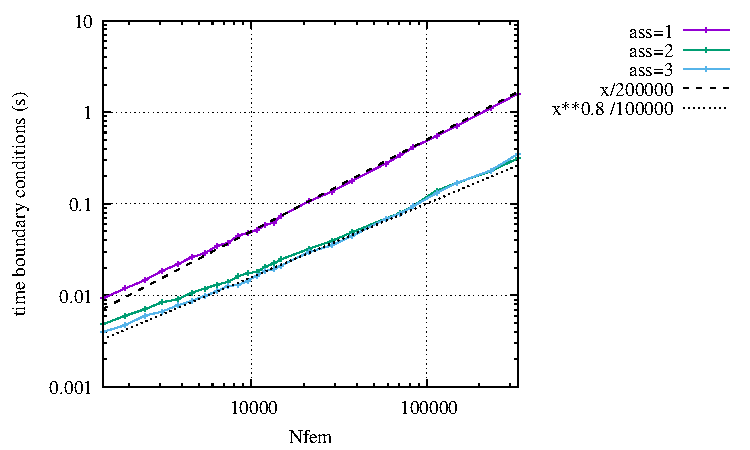
\includegraphics[width=10cm]{python_codes/fieldstone_181/RESULTS/times_bc.pdf}
\end{center}

\item The time needed to convert the matrix to CSR format
\begin{center}
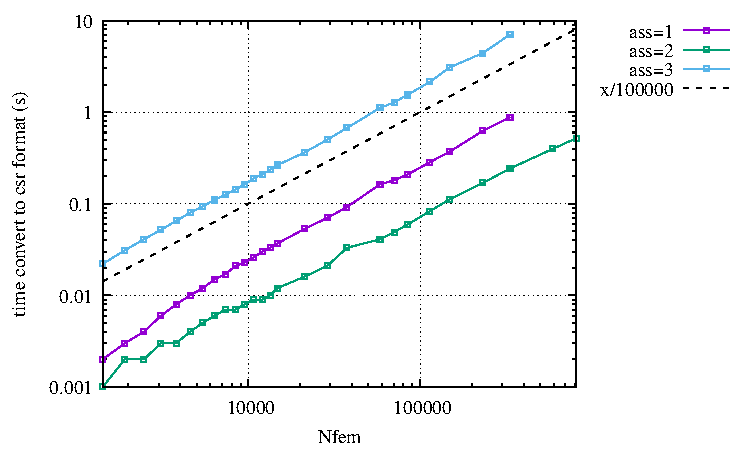
\includegraphics[width=10cm]{python_codes/fieldstone_181/RESULTS/times_convert.pdf}
\end{center}

\item The total time spent building the elemental $\K_e$ and $\G_e$.
\begin{center}
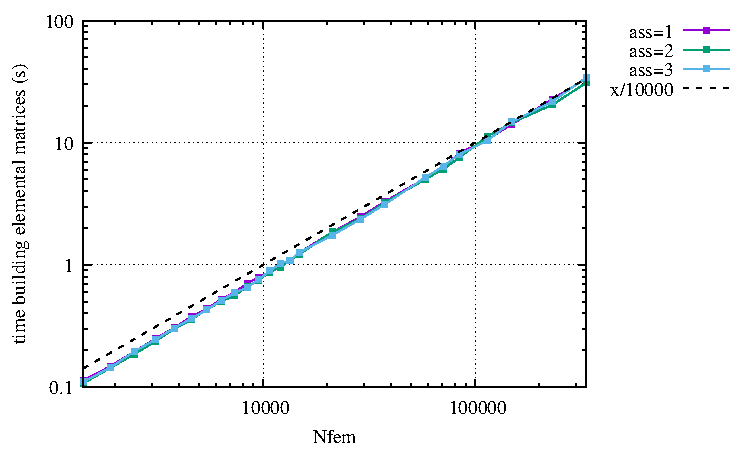
\includegraphics[width=10cm]{python_codes/fieldstone_181/RESULTS/times_matrices.pdf}
\end{center}
Unsurprisingly it is identical across all 3 methods.

\item The time spent solving the linear system
\begin{center}
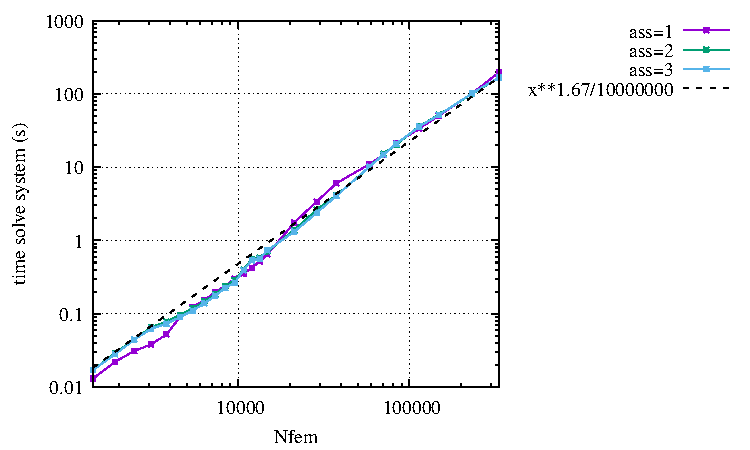
\includegraphics[width=10cm]{python_codes/fieldstone_181/RESULTS/times_solve.pdf}
\end{center}
Unsurprisingly it is identical across all 3 methods.

\end{itemize}

Finally we can verify that the solution for all three methods is identical:
\begin{center}
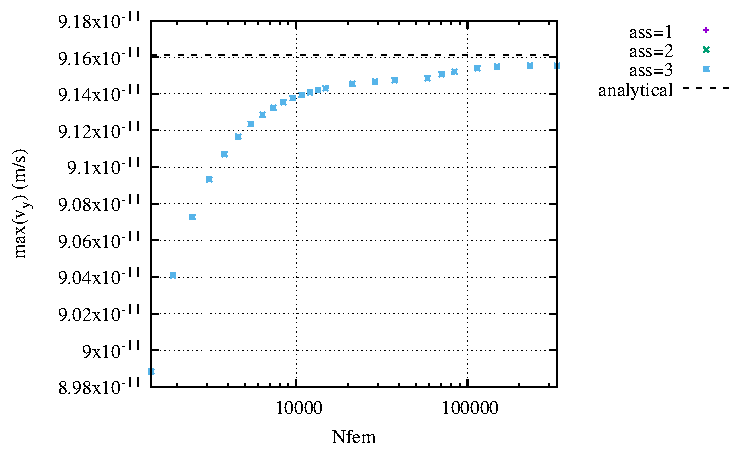
\includegraphics[width=10cm]{python_codes/fieldstone_181/RESULTS/vy}
\end{center}




\noindent 
\includegraphics[width=2.5cm]{./images/conclusion.png}
Method 1 is the slowest. 
Method 2 is the fastest. It requires a bit more work (large additional arrays need to be 
declared and filled) and the time to fill these arrays is not negligible BUT if 
multiple solves are to be carried out (nonlinear iterations, time stepping) these 
arrays do not change and their relative cost becomes then negligible.. 
Method 3 is comparable to method 2 in terms of performance but the conversion to CSR
takes more time (at 128x128 resolution 3s vs 0.1s!). 
Application of boundary conditions for methods 2 and 3 is virtually negligible ($<$0.2s
at 128x128).
Finally, we see that passed a given resolution the solve time will 
come to dominate in all three cases (for example, at resolution 128x128 with method 2
the build time is 15(+5)s while the solve is 46s). 

\begin{center}
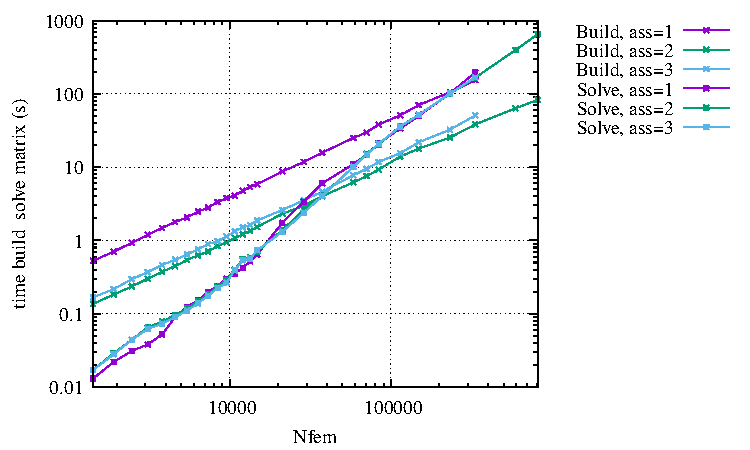
\includegraphics[width=10cm]{python_codes/fieldstone_181/RESULTS/times_build_solve.pdf}
\end{center}


 


